







\section{Numerical Methods}
\subsection{Numerical Discretisation of Spacetime} \label{grchombo:sec:numericaldisc}

The are many ways to numerically time evolve a field theory on some spatial surface. Some popular methods include spectral methods, fourrier methods, finite element models and finite volume methods [MAYBE ADD REFS?]. The method used throughout this work is the finite difference framework. This entails modelling a continuous spacetime with a discrete lattice of points; usually this lattice is cuboidal or cubic. A field $\phi(x^\mu)$ over a manifold $\M$ is expressed as a set of discrete values $\phi^n_{ijk}$, for integer $\{n,i,j,k\}$, where the coordinate $(x^n_{ijk})^\mu = \{n \Delta t, i \Delta x, j \Delta y, k \Delta z \}$ where $\Delta t$, $\Delta x$, $\Delta y$ and $\Delta z$ represent the grid spacing for example in cartesian coordinates. In the limit that the grid spacing tends to zero, the lattice and discretized fields perfectly model the continuum. For a detailed introduction to numerical methods the reader is directed to [REF] [NUMERICAL RECIPES IN C].

To calculate gradients on a lattice, we can consider a two dimensional manifold spanned by coordinates $\{t,x\}$. We can no longer lean on the traditional definition of $\dd f / \dd x$,
\begin{equation}
\frac{\dd f}{\dd x} := \lim_{\Delta x \rightarrow 0} \left( \frac{f(x+\Delta x)-f(x)}{\Delta x} \right),
\end{equation}
as there no longer exists two points $x$ and $x+\Delta x$ that are infinitessimally close to each other. Derivatives are now calculated by comparing gridpoints a finite distance from each other; this requires the well known formula for the taylor expansion of a function about a point $x_0$,
\begin{equation}
f(x) = f(x_0) + (x-x_0) f'(x_0) + \frac{(x-x_0)^2}{2!}f''(x_0) + \frac{(x-x_0)^3}{3!}f'''(x_0) + ... \,. \label{grchombo:eq:taylor}
\end{equation}
To elucidate this idea, a formula for the second derivative we will calculate an expression for the second derivative. Picking five lattice points, equally spaced by $\Delta x$, with coordinates $\{x_{-2},x_{-1},x_{0},x_{1},x_{2}\}$, and writing $f(x_i) = f_i$, we can use Eq.~(\ref{grchombo:eq:taylor}) to write,
\begin{align}
f_{2} &\approx f_0 + 2\Delta x f'_0 + 2 (\Delta x)^2 f''_0 + \frac{4}{3}(\Delta x)^3 f'''_0+ \frac{2}{3} (\Delta x)^4 f''''_0, \\
f_{1} &\approx f_0 + \Delta x f'_0 + \frac{1}{2}(\Delta x)^2f''_0 + \frac{1}{6}(\Delta x)^3f'''_0 + \frac{1}{24}(\Delta x)^4f''''_0,\\
f_0 &\approx f_0 , \\
f_{-1} &\approx f_0 - \Delta x f'_0 + \frac{1}{2}(\Delta x)^2f''_0 - \frac{1}{6}(\Delta x)^3f'''_0 + \frac{1}{24}(\Delta x)^4f''''_0,\\
f_{-2} &\approx f_0 - 2\Delta x f'_0 + 2 (\Delta x)^2 f''_0 - \frac{4}{3}(\Delta x)^3 f'''_0+ \frac{2}{3} (\Delta x)^4 f''''_0,
\end{align}
where the taylor expansion is stopped at terms of order $(\Delta x)^4$. The equations above can be inverted to give,
\begin{equation}
\frac{\dd^2 f}{\dd x^2}\Bigg|_{x_0}:=f''_0 = \frac{-f_2 + 16 f_1 - 30 f_0 + 16 f_{-1} - f_{-2} }{12 (\Delta x)^2}, \label{grchombo:eq:d2fdx2}
\end{equation}
and an approximation for the second derivative using a discrete sum of neighbouring points, also called a stencil, has been obtained. Adding terms of order $(\Delta x)^5$ would not affect the result as the pairs of terms $\{f_2,f_{-2}\}$ and $\{f_1,f_{-1}\}$ appear in equal amounts; therefore Eq.~(\ref{grchombo:eq:d2fdx2}) is correct upto a taylor expansion of order $(\Delta x)^6$. Given that $f''_0$ appears with a $(\Delta x)^2$ and Eq.~(\ref{grchombo:eq:d2fdx2}) is correct untill terms of order $(\Delta x)^6$, then the expression is accurate up to fourth order. [CHECK THIS?] Any other derivate to any order accuracy (in any dimension) can be calculated in a similar fashion. In the limit that the grid spacing $\Delta x \rightarrow 0$ the approximations for the derivatives approach the exact contiuum limit; higher order accurate stencils approach the continuum limit more quickly.


\subsection{Boundary Conditions} \label{grchombo:sec:bc}
Another artefact of evolving field equations over a volume on a computer is that the volume must have finite volume; a computer does not have infinite memory to store an infinite amount of gridpoints. The usual way to deal with this problem is to enforce an algebraic condition on the fields on a surface surrounding the region of interest. Alternatively, an infinite volume can be modeled if coordinates are used which compactify the volume to some finite region, this corresponds to the grid space diverging or resolution becoming infintely low quality towards the boundary.

Common boundary conditions include Dirichlet (fixed value), Von-Neumann (fixed derivative) or some mix of these conditions. When discretising a field theory over a lattice of points, it is more common to re-categorize boundary conditions into types such as reflective, periodic or symmetric.

As an example in one spatial dimension, symmetric boundary conditions for a field $\phi$ about a point $x_n$ could be implemented by creating extra {\it ghost cells} beyond the desired simulation domain with coordinates $\{x_{n+1},x_{n+2},x_{n+3},...\}$ separated by $\Delta x$ and setting,
\begin{align}
\phi_{n+1} = \phi_{n-1}, \quad \phi_{n+2} = \phi_{n-2}, \quad \phi_{n+3} = \phi_{n-3}, \quad ... \, ,
\end{align}  
where $\phi_i = \phi(x_i)$. These extra ghost cells allow the calculation of derivatives at $x_n$ using stencils, as shown in section \ref{grchombo:sec:numericaldisc}; without these ghost cells the stencil would not be able to access points $x_{m}$ where $m>n$. The number of ghost cells should be chosen to be the minimum required to allow the calculation of derivcative stencils at each point in the simulation domain. The desired location of the boundary condition does not have to coincide with a gridpoint. As an example, modifying the symmetric boundary condition to be centered on $x_n + \Delta x /2$ instead results in,
\begin{align}
\phi_{n+1} = \phi_{n}, \quad \phi_{n+2} = \phi_{n-1}, \quad \phi_{n+3} = \phi_{n-2}, \quad ... \, .
\end{align} 

Generic boundary conditions can be imposed by assigning values to ghost cells similarly to above. Although the examples given in this section are in one dimension, the ideas generalise to arbitrary dimensions.


\subsubsection{Sommerfeld Boundary Conditions}
A very useful type of boundary condition is the Sommerfeld boundary condition [REF], used to approximate an outgoing wave being transmitted through the boundary condition. Sommerfeld boundary condtions can be derived from studying the solution to the wave equation in spherical symmetry in flat space,
\begin{equation}
-\frac{1}{v^2}\partial_t^2 \Psi +  \gamma^{ij}\D_i \D_j \Psi = 
-\frac{1}{v^2}\partial_t^2 \Psi +\frac{1}{\sqrt{-\gamma}} \partial_i \left(\sqrt{\gamma} \gamma^{ij} \partial_j \Psi \right) =
-\partial^2_t \Psi + \frac{1}{r^2}\partial_r \left( r^2 \partial_r \Psi\right)=0,
\end{equation}
for some field $\Psi$ with wavespeed $v$. In spherical polar coordinates, $\gamma^{ij}=\mathrm{diag}\{1,r^{-2},r^{-2} \mathrm{cosec}^2(\theta) \}$. It can easily be shown that this has an outgoing wave solution,
\begin{equation}
\Psi(r,t) = \Psi_\infty + \frac{A}{r}\psi(r-vt),
\end{equation}
for an asymptotic value $\Psi_\infty$ and constant $A$. In differential form this can be written as,
\begin{equation}
\frac{1}{v}\partial_t \Psi + \partial_r \Psi+ \frac{1}{r}(\Psi-\Psi_\infty) =0.
\end{equation}
The equation of motion for $\Psi$ can be used to write $\partial_t$ in terms of spatial derivatives and field values giving the new boundary condition which can be applied numerically as a regular mixed type boundary condition. 

In general relativity, Sommerfeld boundary conditions are commonly used with $v=c=1$ (the speed of light) to avoid reflections of matter and gravitational waves from the boundary of a simulation. It should be noted that Sommerfeld boundary conditions are approximate in general relativity for a number of reason. Matter often doesn't propogate at the speed of light, gravitational waves only obey a wave equation in flat space and the Sommerfeld boundary conditions were derived in spherical symmetry and flat space. These conditions are satisfied in the limit the simulation boundary is infinately far away from the centre of an asymptotically flat vacuum spacetime. It has been found experimentally in my work that ensuring the boundary conditions are sufficiently far away from any compact objects is very important in maintaining accuracy of the simulation when using Sommerfeld boundary conditions.


\subsection{The Method of Lines} \label{grchombo:sec:mol}
Assuming adequate boundary conditions are in place, the time evolution of initial data $\phi^n_{ijk}$ covering a spacelike computational grid can be done by applying a time integration scheme to the PDE governing the field $\phi(x^\mu)$. There are many ways to do this and the reader is directed to [REF] [NUMERICAL RECIPES IN C] for a comprehensive introduction. A common and simple method is the method of lines (MoL). The MoL reduces the dimensionality of the PDE problem to set of ODE's in time at each fixed coordinate and treats spatial derivatives as a function on this line through spacetime. For example, consider the partial differential equation,
\begin{equation}
\partial_t \phi(\bs{x},t) = \hat{{O}} \phi(\bs{x},t) + f(\phi,\bs{x},t),
\end{equation}
where $\hat{{O}}$ is some spatial derivative operator, $f$ is a function and $\bs{x}$ are spacelike coordinates. In the MoL the operator $\hat{{O}}$ can be discretised on a grid like,
\begin{equation}
\hat{{O}} \phi (\bs{x},t) \rightarrow ({O} \phi)_{ijk}(t),
\end{equation}
where $({O} \phi)_{ijk}(t)\approx \hat{O} \phi (x_{ijk},t)$ is a sum of field values at neighbouring gridpoints generated by the method of finite differences. Discretising the function $f$ on the grid gives the following ODE for each gridpoint with spatial indeces $\{i,j,k\}$,
\begin{equation}
\partial_t \phi_{ijk}(t) = (\hat{O} \phi)_{ijk}(t) + f_{ijk}(\phi,t) = {F}_{ijk}(\phi,t), \label{grchombo:eq:MoL}
\end{equation}
where ${F}_{ijk}(\phi,t)$ can be treated as the discretisation of a continuum function ${F}(\phi,\bs{x},t)$. 

\subsection{Integration of ODE's}
To perform the time evolution of the ODE Eq.~(\ref{grchombo:eq:MoL}), one now needs to pick a time integration method for an ODE (rather than a PDE if MoL was not used). The obvious choice might be to discretise the time integral like,
\begin{equation}
\partial_t \phi^n_{ijk} = \frac{\phi^{n+1}_{ijk} - \phi^n_{ijk}}{\Delta t},
\end{equation} 
where $\Delta t$ is the time-step of evolution. This can be substituted into Eq.~(\ref{grchombo:eq:MoL}) to give,
\begin{equation}
\phi^{n+1}_{ijk} = \phi^n_{ijk} + {F}^n_{ijk}  \Delta t, \label{grchombo:eq:eulermethod}
\end{equation} 
which is an explicit scheme; the desired object $\phi^n_{ijk}$ is given by an explicit formula. This is known as the Eular method and is often unstable; it can be shown to be completely unstable no matter how small $\Delta t$ is taken to be for $F^n_{ijk} = A \phi^n_{ijk}$ for positive constant $A$. There is nothing stopping us instead writing,
\begin{equation}
\phi^{n+1}_{ijk} -  {F}^{n+1}_{ijk} \Delta t = \phi^n_{ijk},
\end{equation} 
which is known as an implicit scheme as the desired object $\phi^{n+1}_{ijk}$ is given by an implicit equation. This is called the backwards Eular method and is often stable, but only first order accurate in time. This can be improved to the second order accurate Crank-Nicolson method,
\begin{equation}
\phi^{n+1}_{ijk} -  \frac{1}{2}{F}^{n+1}_{ijk} \Delta t = \phi^n_{ijk} +  \frac{1}{2}{F}^{n}_{ijk} \Delta t, \label{grchombo:eq:crank}
\end{equation} 
but is still implicit in $\phi^n_{ijk}$. These problem with implicit methods is that the $F^{n+1}_{ijk}$ are some combination of $\phi^{n+1}_{ijk}$ and multiple other neighbouring gridpoints to $\{i,j,k\}$; the number of gridpoints increases with higher order accurate spatial derivatives. Solving the set of simultanious equations in Eq.~(\ref{grchombo:eq:crank}), for example, requires the inverting of a very big (albeit sparse) matrix whose size scales with the number of gridpoints. This can be done in a single step if the $F^n_{ijk}$ are linear in $\phi^n$. For non-linear ODE's the $F^n_{ijk}$ are non-linear in $\phi^n_{ijk}$; in the best case one can linearise if and the $\phi^{n+1}_{ijk}$ can be solved with an iterative method, in the worst the implicit scheme is impossible to solve.

A stable and explicit method can be obtained by seeking a higher order accurate time derivative. In a similar fashion to the derivation of Eq.~(\ref{grchombo:eq:d2fdx2}), one can write,
\begin{align}
\phi^n_{ijk} &= \phi^n_{ijk},\\
\phi^{n-1}_{ijk} &= \phi^n_{ijk} - \Delta t \dot{\phi}^n_{ijk} + \frac{1}{2}(\Delta t)^2 \ddot{\phi}^n_{ijk},\\
\phi^{n-2}_{ijk} &= \phi^n_{ijk} - 2\Delta t \dot{\phi}^n_{ijk} + 2(\Delta t)^2 \ddot{\phi}^n_{ijk},
\end{align}
where the dot represents a time derivative and the taylor expansion has been given up to $(\Delta t)^2$ terms. Rearranging, these give
\begin{equation}
\partial_t \phi^n_{ijk} = \frac{-3 \phi^n_{ijk} + 4 \phi^{n-1}_{ijk} - \phi^{n-2}_{ijk}}{6 \Delta t}. \label{grchombo:eq:hmmmmm}
\end{equation}
Substituting this into Eq.~(\ref{grchombo:eq:MoL}) gives an explicit equation for $\phi^n_{ijk}$,
\begin{equation}
\phi^n_{ijk} = \frac{4}{3}\phi^{n-1}_{ijk} - \frac{1}{3}\phi^{n-2}_{ijk} - 2 F_{ijk} \Delta t,
\end{equation}
where the index $n$ has been omitted from $F_{ijk}$ as is can be replaced with any combination of $F^n_{ijk}$, $F^n_{ijk}$ and $F^n_{ijk}$ such as $F^n_{ijk} = \frac{4}{3}F^{n-1}_{ijk}-\frac{1}{3}F^{n-2}_{ijk}$. Even thought this method is explicit it requires two sets of initial data, $\phi^{n-1}_{ijk}$ and $\phi^{n-2}_{ijk}$. 

MAYBE CUT THIS BIT SHORT AT EQ \ref{grchombo:eq:hmmmmm} 

\subsubsection{The Runge Kutta Method} \label{grchombo:sec:rk4}
The Runge-Kutta method is an explicit ODE integration scheme that can be made accurate to arbitrary order in $\Delta t$. For an ODE like
\begin{equation}
\frac{\dd \phi}{ \dd t} + F(\phi,t),
\end{equation}
the widely used fourth order accurate Runge-Kutta (RK4) method first calculates four intermediate gradients $\{k_1,k_2,k_3,k_4\}$,
\begin{align}
k_1 &=  F(\phi,t) ,\\
k_2 &=  F(\phi + \frac{1}{2}k_1 \Delta t,t+ \frac{1}{2} \Delta t) ,\\
k_3 &=  F(\phi + \frac{1}{2}k_2 \Delta t,t+ \frac{1}{2} \Delta t) ,\\
k_4 &=  F(\phi + k_3 \Delta t,t+  \Delta t) ,
\end{align}
that are summed in a way that calculates $\phi(t+\Delta t)$ from $\phi(t)$,
\begin{equation}
\phi(t+\Delta t) = \phi(t) + \frac{1}{6}\left( k_1 + 2k_2 + 2k_3 + k_4\right)\Delta t + \mathcal{O}(\Delta t^5),
\end{equation}
which removes errors upto and including $(\Delta t)^4$ terms. A similar procedure can be done for any desired accuracy with higher order methods becoming quite involved. The simplicity of this RK4 scheme along with it's robustness in use has no doubt led to it being the go-to method for integrating ODEs. Lower order Runge-Kutta methods exist such as RK1 which is the Eular method in Eq.~(\ref{grchombo:eq:eulermethod}).



\section{GRChombo}
\subsection{Overview of GRChombo}

GRChombo [REF] [JOSS AND OLD PAPER] is an open-source fully non-linear Numerical Relativity (NR) code built on top of Chombo [REF], a PDE solver with adaptive mesh refinement (AMR). GRChombo is written in C++ making extensive use of templating, classes and object oriented programming. GRChombo also supports vectorisation and parallelisation with OpenMP and MPI making it scale efficiently to large problems suitable for use on supercomputer clusters. Current public examples of GRChombo include a black hole binary with seperate spins, a single kerr black hole and a compact real scalar configuration. 

The AMR in Chombo relies on the Berger-Oliger style AMR [REF] with block-structured Berger-Rigoutsos grid generation [REF]. The labelling of which regions to regrid, called tagging, is specifiable by the user; a common example to use a variable $\psi$ to make a new, gradient sensitive variable 本$\aleph$,
\begin{equation}
\aleph = \Delta x \sqrt{\frac{\left| \sum_{ij}(\partial_i\partial_j \psi )(\partial_i\partial_j \psi)\right|}{\left|\sum_{k} (\partial_k \psi )(\partial_k \psi)\right|+\epsilon}},
\end{equation}
for grid spacing $\Delta x$ and small positive $\epsilon$ to avoid division by zero. Some threshold $\psi_0$ is prespecified and any gridpoint where $\aleph > \psi_0$ is flagged for regridding. The reason for premultiplying by $\Delta x$ is so that as the grid spacing gets smaller on more deeper levels the tagging criterion is not flagged unless gradients become more extreme.

In order to evolve a spatial hypersurface with the Einstein equation, GRChombo uses either the BSSN formalism [REF] described in section \ref{nr:sec:bssn} or the CCZ4 formalism [REF]. A summary of the CCZ4 formulation is given in section \ref{nr:sec:ccz4} along with the equations of motion used in this work. The conformal factor used is $\chi = \gamma^{-\frac{1}{3}}$ where $\gamma$ is the metric determinant from Eq.~(\ref{nr:eq:gammaij}) on the three dimensional hypersurface $\Sigma_t$. The time evolution scheme is the method of lines \ref{grchombo:sec:mol} using 4th order spatial derivatives \ref{grchombo:sec:numericaldisc} and runge kutta 4th order time integration \ref{grchombo:sec:rk4}. While 6th order spatial derivatives have been implemented, they are not used in this work due to their increasing the number of ghost cells needed. Kreiss-Oliger dissipation [REF] is used to dampen high frequency noise occuring from interpolation, regridding of AMR and high field gradients inside black hole regions. As described in section \ref{nr:sec:gaugeconditions}, the moving puncture gauge with conformal factor $\chi$ is used to evolve moving black hole singularities.

The code can implement Sommerfeld, periodic, reflective and extrapolating boundary conditions. Simulations in this work all use some combination of Sommerfeld boundary conditions for boundaries far away and reflective boundary conditions in a plane of symmetry. Headon collision of the same object can use {\it octant} symmetry, three planes of symmetry on the planes $x=0$, $y=0$ and $z=0$. This means one only needs to simulate the region $x>0$, $y>0$ and $z>0$ with reflective boundary conditions on the symmetry planes; the overall problem size (or number of gridpoints) reduces by a factor of eight. Similarly, headon collisions of non-similar objects can use {\it quadrant} symmetry, reducing the problem size by four. A general inspiral of two dissimilar compact obejcts has one plane of symmetry, the plane of inspiral; {\it bitant} symmetry can be used to half the problem size. For all the pre-mentioned symmetries, a suitable rest frame must be used aligning with the symmetries of the initial data. For detail on numerical implementation of boundary conditions see section \ref{grchombo:sec:bc}.

A selection of diagnostic tools have been included into GRChombo. These include, but are not limited to, black hole horizon finders, gravitational wave extraction and the calculation for ADM mass and momentum, Noether charges and energy-momentum densities and fluxes. The diagnostic for the angular momentum density and flux are the result of section \ref{q:sec:q}.


While GRChombo can be used to simulate traditional spacetimes, such as binary black hole inspirals [REF] [REF MIREN PAPER], it excells at simulating novel and theoretical physics due to its adaptable code and AMR. The advantage of AMR is that regions needing higher resolution are assigned (and de-assigned) dynamically during run time; this requires no a-priori knowledge or pre-determined grid structure unlike other NR codes. [DO I LIST CODES HERE?] AMR is especially useful for matter simulations that can develop features requiring higher resolution in places a human may not expect making pre-specified mesh refinement hard to use. GRChombo has also sucessfully simulated ring-like configurations [REF] [Thomas,Josu] and inhomogeneous spacetimes [REF] [ref pau katy ...] which would be tricky with a conventional pre-specified grid structure. GRChombo has been designed to be straight forward to modify making it an excellent choice for exotic matter, modified gravity theories and higher dimensional spacetimes.


\subsubsection{Simulation Units}
MAKE THIS WORK WITH THE CONVENTIONS SECTION ASND THEN DESCRIBE WHAT IS NEW FOR ONLY THE SIMULATIONS

GRChombo defaults to geometric units, as described in section (1.2). The scalar field $\vp$ appears in the action as
\begin{equation} S = \int_{\M} \left[g^{\mu\nu}\partial_\mu \vp \partial_\nu \vp^* + ... \right]\dd x^4\end{equation}
and given $S$ and the metric are dimensionless, dimensional analysis tells us $\vp$ has units of inverse length in natural units, or units of energy. The Klein-Gordon mass $m$
\begin{equation} \Box \vp = m^2 \vp\end{equation}
can be absorbed into new dimensionless spatial coordinates $\tilde{x}^i = x^i m$ changing the KG equation to the scale invariant form.
\begin{equation} \Box \vp = \vp\end{equation}




\subsection{Boson Star Initial Data}

Following on from the EKG ODE's in Eqs.~(\ref{boson:eq:EKGODE1}),  (\ref{boson:eq:EKGODE2}) and (\ref{boson:eq:EKGODE3}) we now seek to solve them numerically to obtain initial data for a single static boson star. The system can be reduced to a set of five first order ODE's with five boundary conditions. For a physical star we would like to impose $\Phi(0) = \Phi_c$, $\Phi'(0)=0$, $\Phi(r\rightarrow\infty)\rightarrow0$, $\Omega'(0)=0$, $\Omega(r\rightarrow\infty)\rightarrow1$, $\Psi'(0)=0$ and $\Psi(r\rightarrow\infty)\rightarrow1$ to be regular at the origin and match the Schwarzschild vacuum solution at large radius; however this is seven boundary conditions and we can only impose five. The condition $\Omega(0)'=0$ cannot be specified as Eq.~(\ref{boson:eq:EKGODE1}) is first order in derivatives of $\Omega$ but given that $r$ and $\Psi'$ both vanish at the origin then $\Omega'$ must also vanish at the origin automatically. One more boundary condition can be removed by asking for the boson star solution to match the isotropic Schwarzschild solution in Eq.~(\ref{intro:eq:iso_bh}) and therefore,
\begin{equation}
\Omega = \left(\frac{1-\frac{m}{2r}}{1+\frac{m}{2r}}\right) \quad \& \quad \Psi = \left( 1+\frac{m}{2r}\right)^2 \end{equation} 
where $m$ can be interpreted as the mass of the boson star; this mass will not enter the boundary condition so can be safely ignored. Combining the two equations above gives
\begin{equation} 
\sqrt{\Psi}\left(1+\Omega\right) = 2
\end{equation}
for a vacuum spacetime. Imposing the single condition $\sqrt{\Psi(\infty)}\left(1+\Omega(\infty)\right)=2$, rather than both $\Omega(\infty)=1$ and $=\Psi(\infty)=1$, then gives asymptotic flatness in just one boundary condition. One final point of importance is the frequency $\omega$ turns the Klein-Gordon ODE into an eigenvalue problem, admitting only discrete values of $\omega$. 

The problem has now been reduced to five ODE's with the following five boundary conditions,
\begin{equation} \{\Phi(0),\Phi'(0),\Psi'(0),\Omega(0),\sqrt{\Psi(\infty)}\left(1+\Omega(\infty)\right);\omega \} = \{ \Phi_c,0,0,\omega_0,2;\omega_0\},\end{equation}
subjected to the condition of an eigenvalue $\omega=\omega_0$. The first attempt to find the radial profile $\{\Phi(r), \Omega(r), \Psi(r)\}$ of the boson star was to use a relaxation 
method [REF] as it trivially incorporates the above two-point boundary conditions. In practice this method did not work well with the eigenvalue problem in $\omega$.
Unlike with a shooting method, there was no obvious way of telling whether the guess $\omega$ was larger or
smaller than the correct value. Even if this problem were overcome, a numerical solution with relaxation is computationally slow, even with Successive Over-Relaxation [REF] [20]; perhaps a multigrid method could work here but a simpler method was used.


\subsubsection{Shooting Method}

To find the initial data for a single Boson star, a private {c++} script was written using RK4 [REF] to integrate the EKG system taking five initial conditions, and eigenvalue guess $\omega_0$, 
\begin{equation} \{\Phi(0),\Phi'(0),\Psi(0),\Psi'(0),\Omega(0);\omega \} = \{ \Phi_c,0,\Psi_c,0,\omega_0;\omega_0\}.\end{equation}
Unfortunately $\omega_0$ and $\Psi_c$ are unknown apriori, but guessing any values reasonably close to untity, such as $\omega_0=0.5$ and $\Psi_c=2$, still give a boson star. This will generally result in the following asymptotic metric,
\begin{equation} g_{\mu\nu}(r\rightarrow\infty) \rightarrow \mathrm{diag}(-A^2,B^2,B^2,B^2), \label{grchombo:eq:ABBB}\end{equation}
 for constant $A$ and $B$. 

 Before we discuss how to find the correct value of $\omega$, there is a subtle numerical problem to adress. Using spherical polar coordinates in flat space, the Klein-Gordon equation (\ref{boson:eq:KGeqn}) with $V=m^2 |\vp|^2$ and ansatz $\vp =\Phi_{flat}(r)e^{\mathrm{i}\omega t}$ reduces to,
\begin{align}
\frac{1}{\sqrt{-g}} \partial_\mu \left(\sqrt{-g} g^{\mu\nu} \partial_\nu \right)\vp &= \frac{\partial V}{\partial |\vp|^2} \vp ,\\
 \partial_t \left( g^{tt} \partial_t \right)\Phi_{flat}(r)e^{\mathrm{i} \omega t} + \frac{1}{r^2} \partial_r \left(r^2 g^{rr} \partial_r \right)\Phi_{flat}(r)e^{\mathrm{i} \omega t} &= m^2 \Phi_{flat}(r)e^{\mathrm{i} \omega t} ,\\
  \omega^2 \Phi_{flat}(r) + \frac{1}{r^2} \partial_r \left(r^2  \partial_r \right)\Phi_{flat}(r) &= m^2 \Phi_{flat}(r) ,\\
\end{align}
where $\sqrt{-g} = r^2 \sin(\theta)$, $g^{tt}=-1$ and $g^{rr}=1$. This has general solution,
\begin{equation}
\Phi_{flat}(r) = \frac{1}{r}\left(C_1 e^{- r \sqrt{m^2-\omega^2}} + C_2 e^{ r \sqrt{m^2-\omega^2}} \right),
\end{equation}
for $\Phi_{flat}(r)$ and two constants $C_1$ and $C_2$. Due to finite resolution during numerical integration, at large radius $C_2$ will never be exactly zero and will eventually grow (along increasing radius) and spoil the numerical integration; even though this behavour was derived in flat space it is still present in curved space with spherical symmetry - especially at such large radius that space is approximately flat. In practice, the scalar field $\Phi$ will decay to some value roughly twenty orders of magnitude smaller than the central density $\Phi(0)$ and is effectively zero within numerical noise. At this point the coefficient $C_2$ is excited by noise and starts to grow exponentially. At a radius $r_*$ when the growing mode is deemed to be dominating, usually detected by an axis crossing $(\Phi(r_*)=0$ or a turning point $\Phi'(r_*)=0)$ the conditions $\Phi(r>r_*)=\Phi'(r>r_*)=0$ are enforced during integration. This creates a vacuum for $r>r_*$ and the spacetime is pure Schwarzschild. After this point, an exponentially growing stepsize was used to reach radii of order $10^8$ to $10^{10}$ times larger than desired for evolutions and the values $A = \Omega_\infty= \sqrt{-g_{00}}$ and $B=\Psi_{\infty}=\sqrt{g_{ii}}$ can be read off.

Interval bisection was used to find the best value of $\omega$, $\omega_0$, to machine precision; for the ground state we can tell that $\omega>\omega_0$ if $\Phi(r)$ develops a turning point before an axis crossing and $\omega < \omega_0$ if $\Phi(r)$ develops an axis crossing before a turning point. To find the $n$'th excited state, which has $n$ axis crossing for $\Phi(r)$ and $\Phi(r\rightarrow \infty) \rightarrow 0$ a similar scheme is followed to find the eigenvalue $\omega_n$. If $\Phi(r)$ has $n+1$ axis crossings then $\omega>\omega_n$ and if $\Phi(r)$ has $n$ axis crossings followed by a turning point then $\omega<\omega_n$. This method of doing a numerical integration and iteratively restarting to get closer to the target solution is known as a shooting method.

Putting everything together, a boson star solution with eigen value $\omega_0$ (or $\omega_n$ for excited stars) and asymptotic metric Eq.~(\ref{grchombo:eq:ABBB}) can be obtained. To find a star with asymptotic metric $\eta_{\mu\nu}$ of flat space, the initial conditions are iteratively improved like $\Omega_c \rightarrow \Omega_c / \Omega_\infty$ and $\Psi_c \rightarrow \Psi_c / \Psi_\infty$; the interval bisection for $\omega$ is then restarted. This is iterated three to five times which leaves $A=\Omega_\infty=1$ and $B=\Psi_\infty=1$ to extreme precision and the isotropic boson star is created. This whole process requires a few seconds runtime for a high resolution 200,000 grid-point simulation on a regular laptop.




%   \begin{figure}[h!]
%   \caption{Boson Star radial profile, Left: Ground state, Right: 1st Excited state}
%   \centering
%   \subfloat{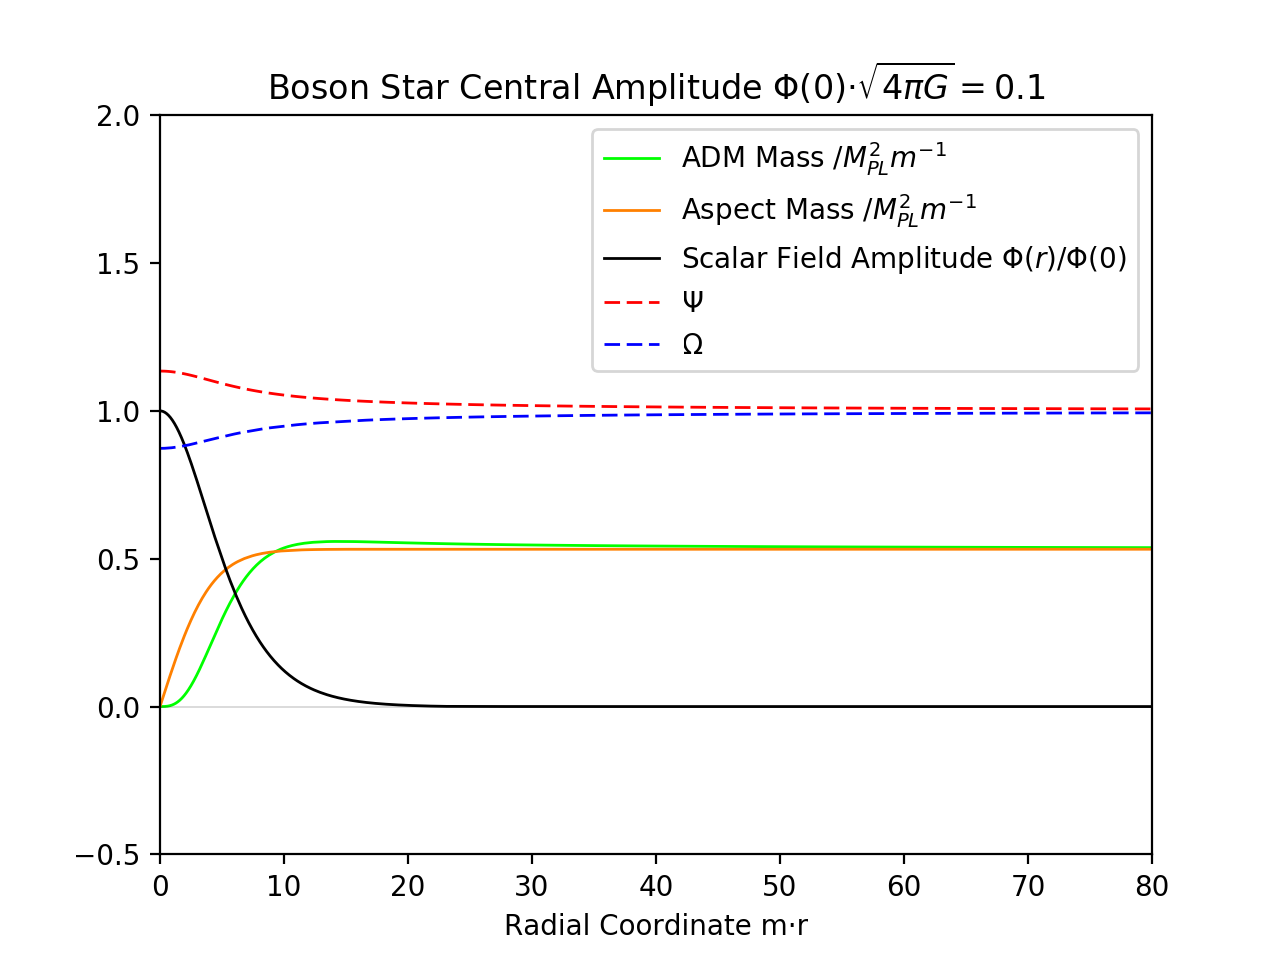
\includegraphics[width=0.5\textwidth]{png/bosonstar_groundstate.png}\label{boson:fig:f1}}
%   \hfill
%   \subfloat{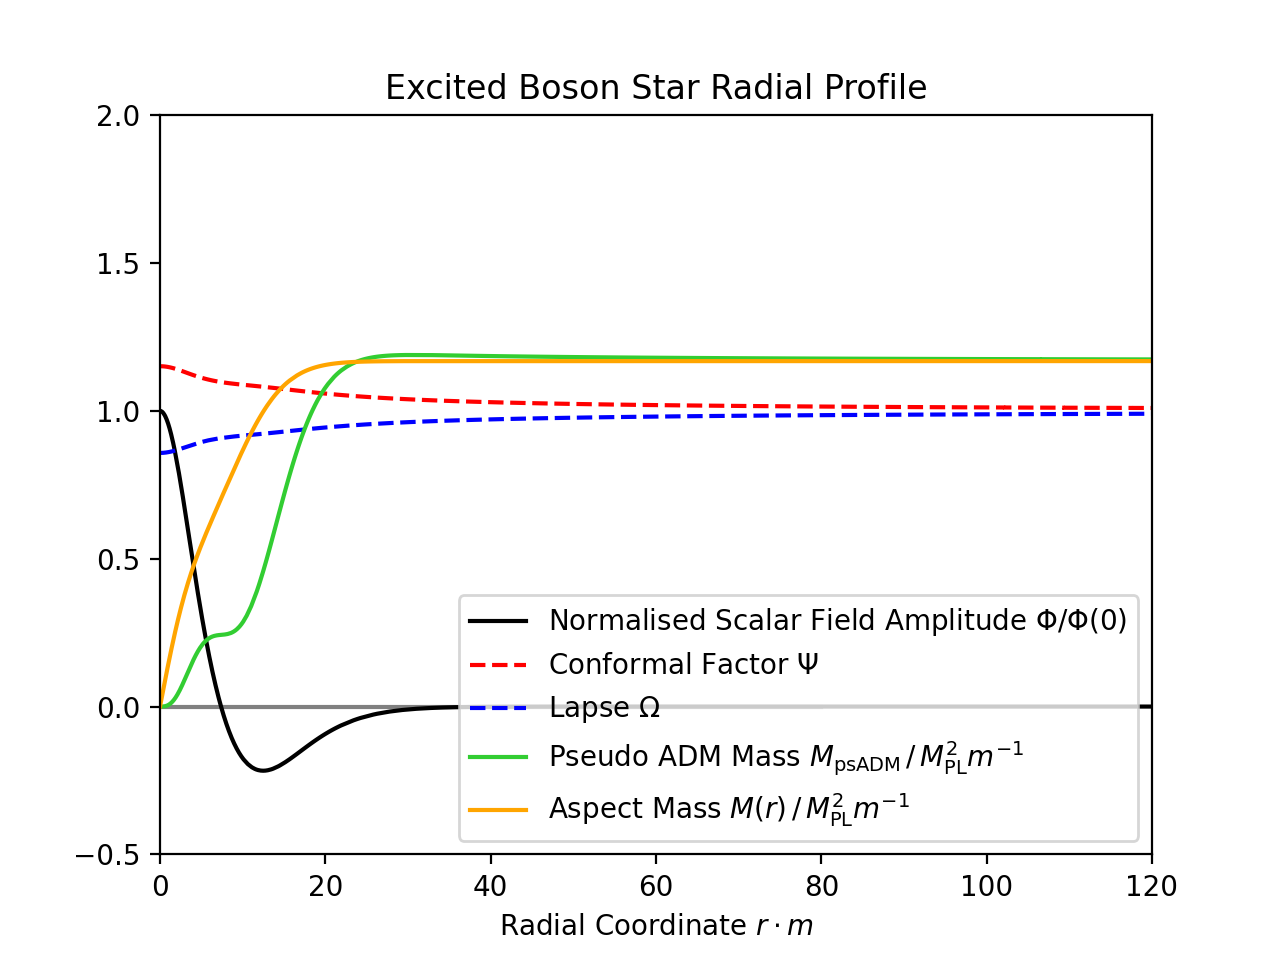
\includegraphics[width=0.5\textwidth]{png/bosonstar_excitedstate.png}\label{boson:fig:f2}}
% \end{figure}

  \begin{figure}[h!]
  \caption{Boson star radial profile for the ground state}
  \centering
  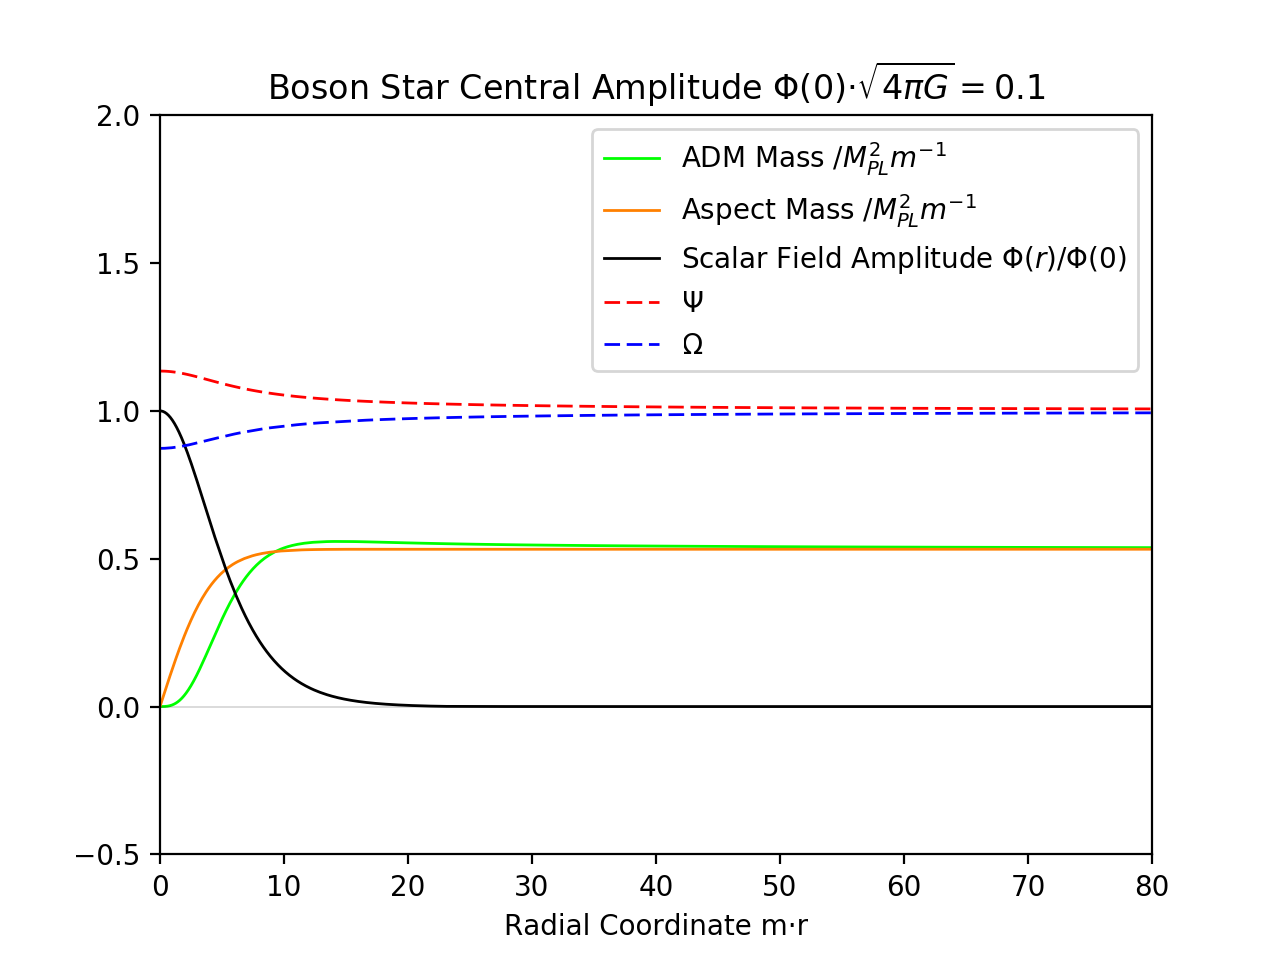
\includegraphics[width=0.8\textwidth]{png/bosonstar_groundstate.png}\label{boson:fig:f1}
\end{figure}

  \begin{figure}[h!]
  \caption{Boson Star radial profile : 1st Excited state}
  \centering
  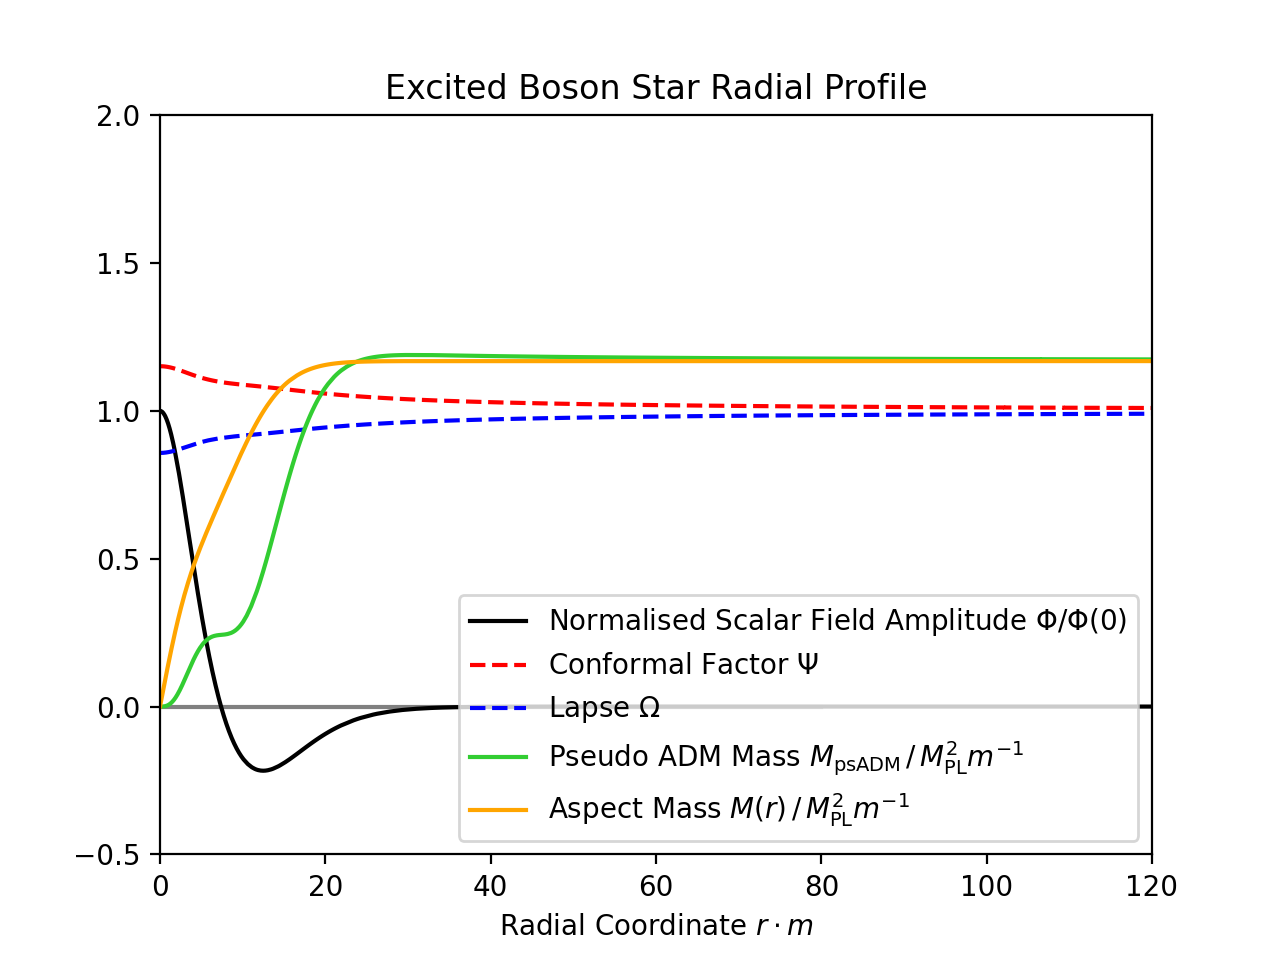
\includegraphics[width=0.8\textwidth]{png/bosonstar_excitedstate.png}\label{boson:fig:f2}
\end{figure}

Figures~\ref{boson:fig:f1} and \ref{boson:fig:f2} show the numerical result for the radial profile of a mini boson star ($\Lambda=0$) and an excited mini boson star. Note two mass definitions are plotted; the ADM mass (calculated as a function of finite r) and the aspect mass $M_A(r)$ which corresponds to assuming the metric's solution is Schwarzschild with $M_A(r)$ rather than $M$. Polytropic fluid stars were also simulated as a preliminary test of the code; they are much easier to create not needing to solve an eigenvalue problem and don't have an asymptotically growing mode. Figures () show how the ADM mass of boson stars varies with central amplitude $\Phi(0)$ and $r_{99}$, the radius which $\Phi(r_{99}) = \Phi(0)/100$. It should be noted that the $\Lambda =0$ case agrees with the known maximum mass, the Kaup limit [] $M_{max} \approx 0.633 {M_{PL}^2}{m^{-1}}$ with the highest measured mass being $ M_{max} = 0.63299(3) {M_{PL}^2}{m^{-1}} $ corresponding to a central amplitude of $\ \sqrt{4\pi G}\Phi(0)_{max} = 0.271(0)$. 

%   \begin{figure}[h!]
%   \caption{Boson star trends, Left: ADM mass vs $\Phi(0)$, Right: ADM mass vs $r_{99}$}
%   \centering
%   \subfloat{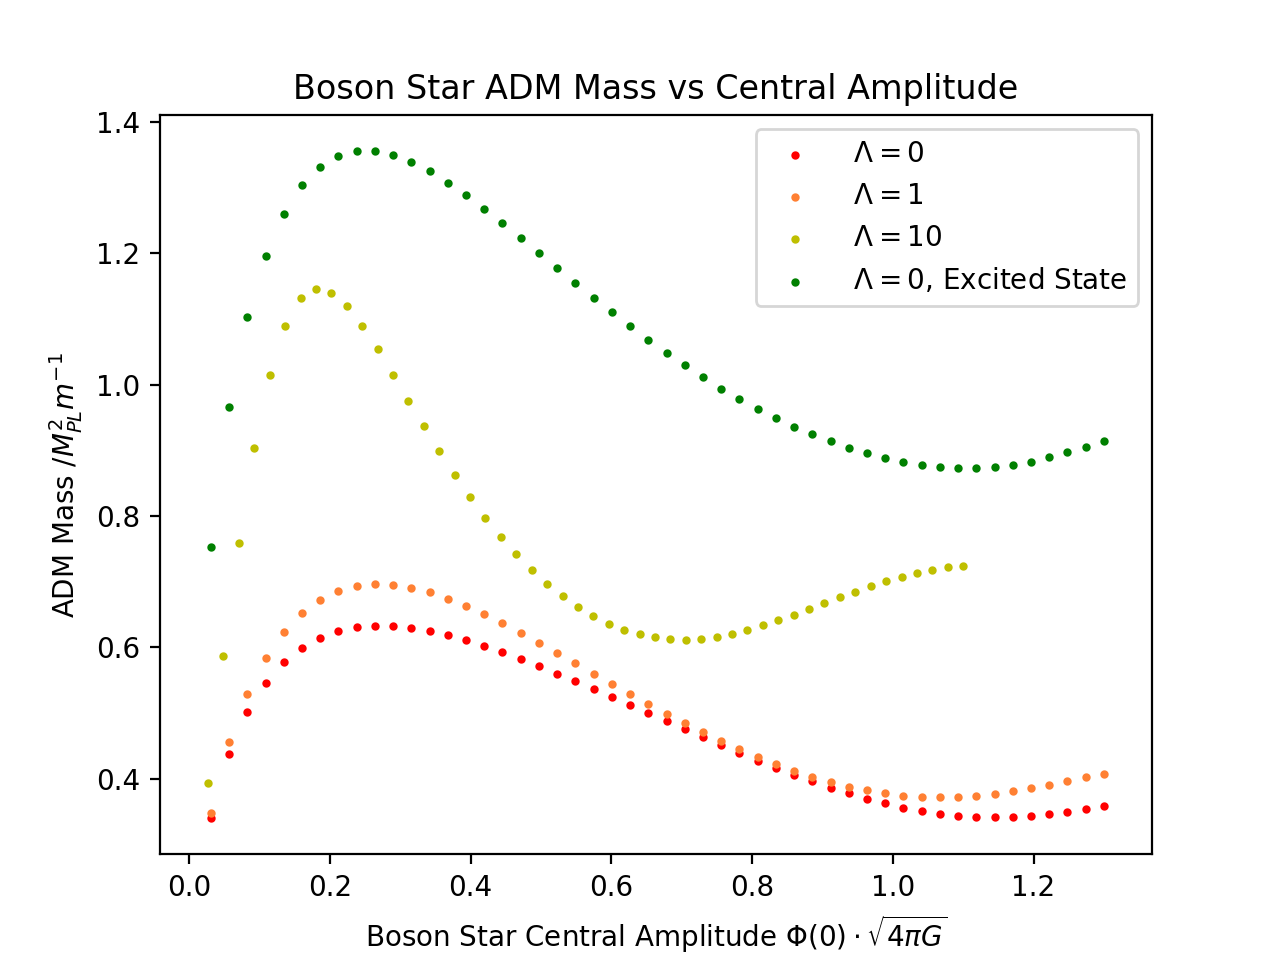
\includegraphics[width=0.5\textwidth]{png/ADM_vs_PC.png}\label{boson:fig:f3}}
%   \hfill
%   \subfloat{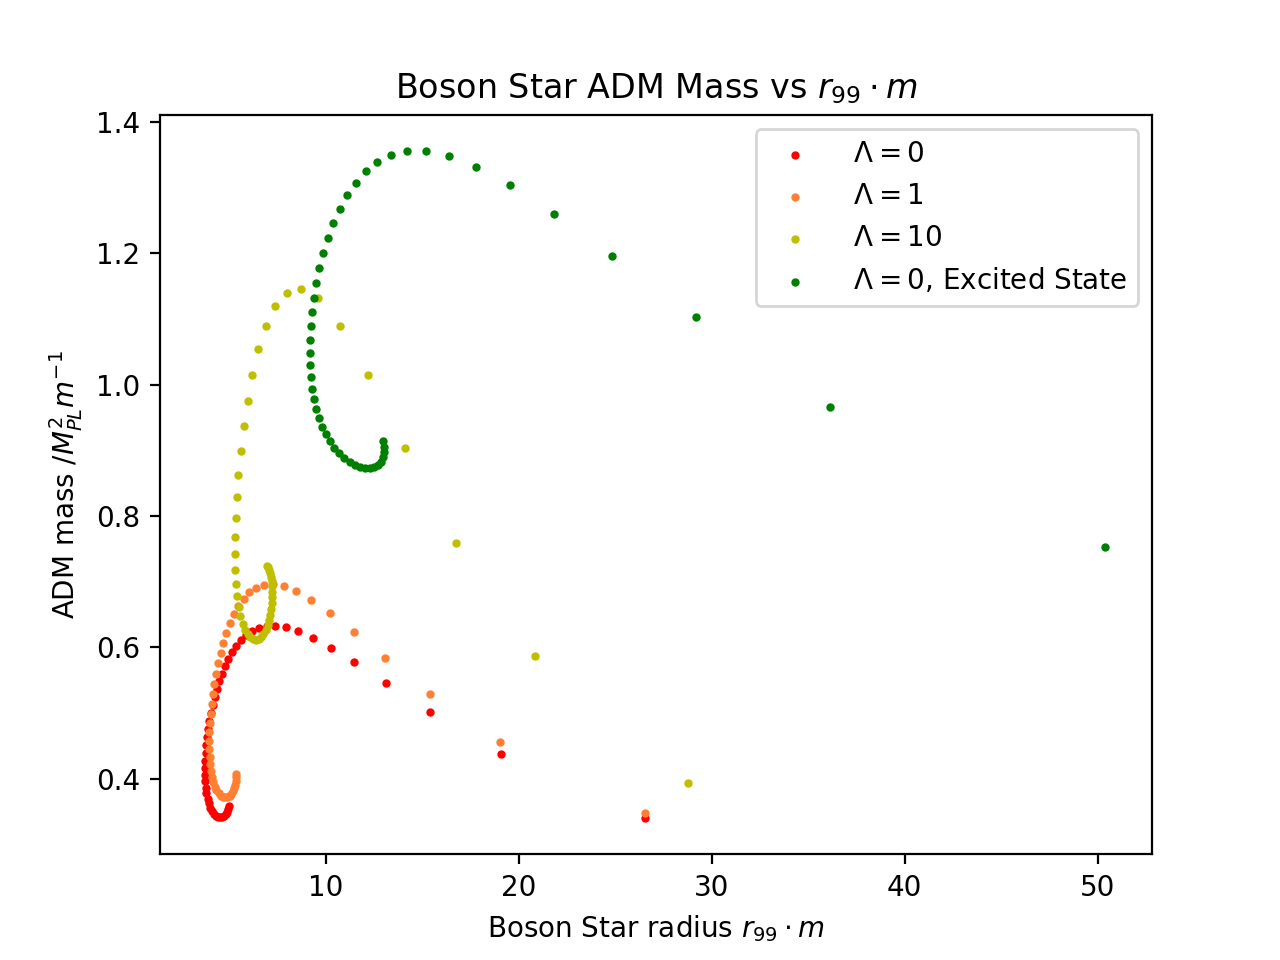
\includegraphics[width=0.5\textwidth]{png/ADM_vs_r99.png}\label{boson:fig:f4}}
% \end{figure}

  \begin{figure}[h!]
  \caption{ADM mass vs $\Phi(0)$}
  \centering
  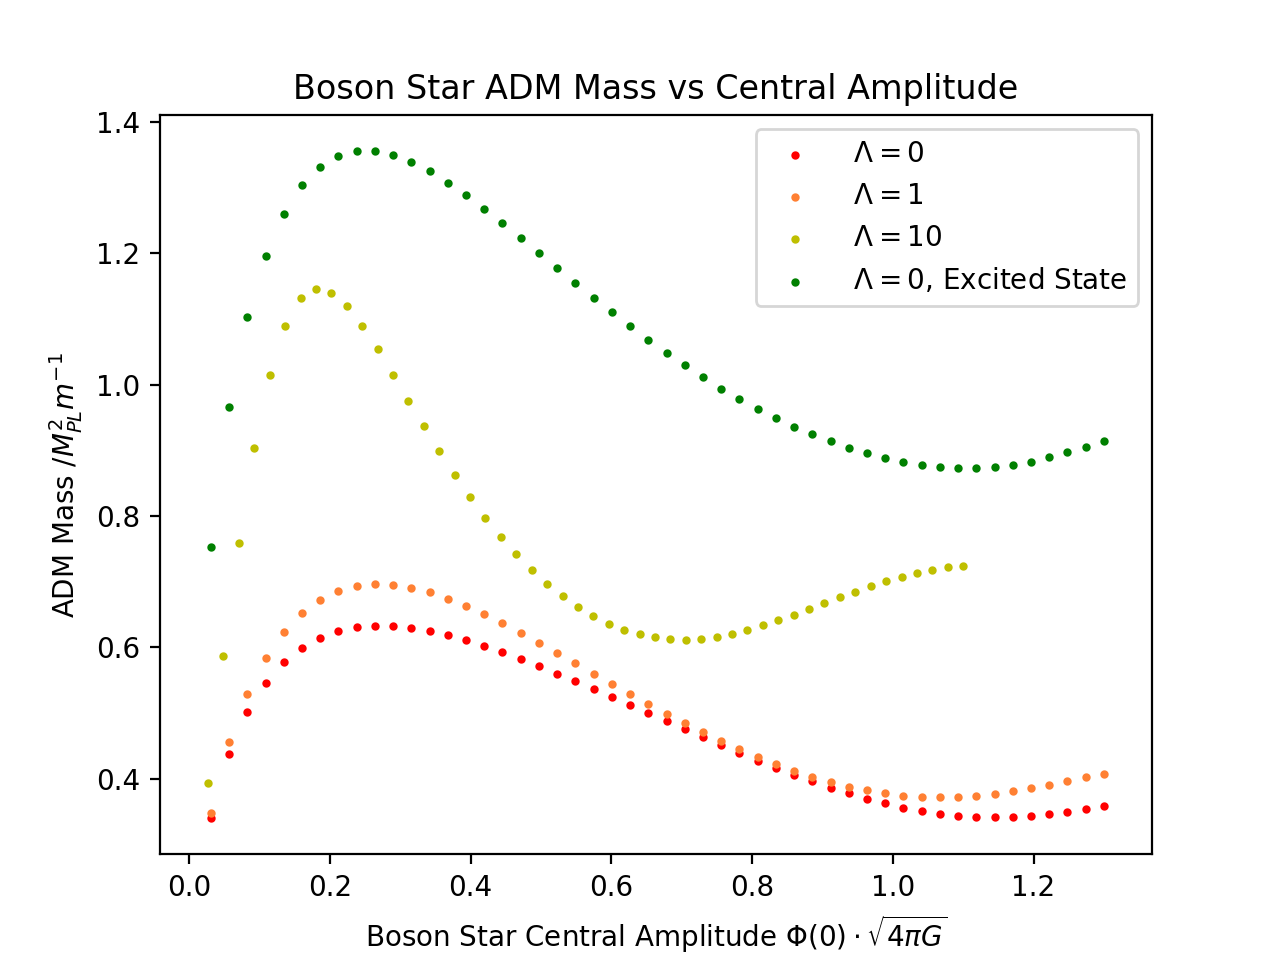
\includegraphics[width=0.8\textwidth]{png/ADM_vs_PC.png}\label{boson:fig:f1}
\end{figure}

  \begin{figure}[h!]
  \caption{ADM mass vs $r_{99}$}
  \centering
  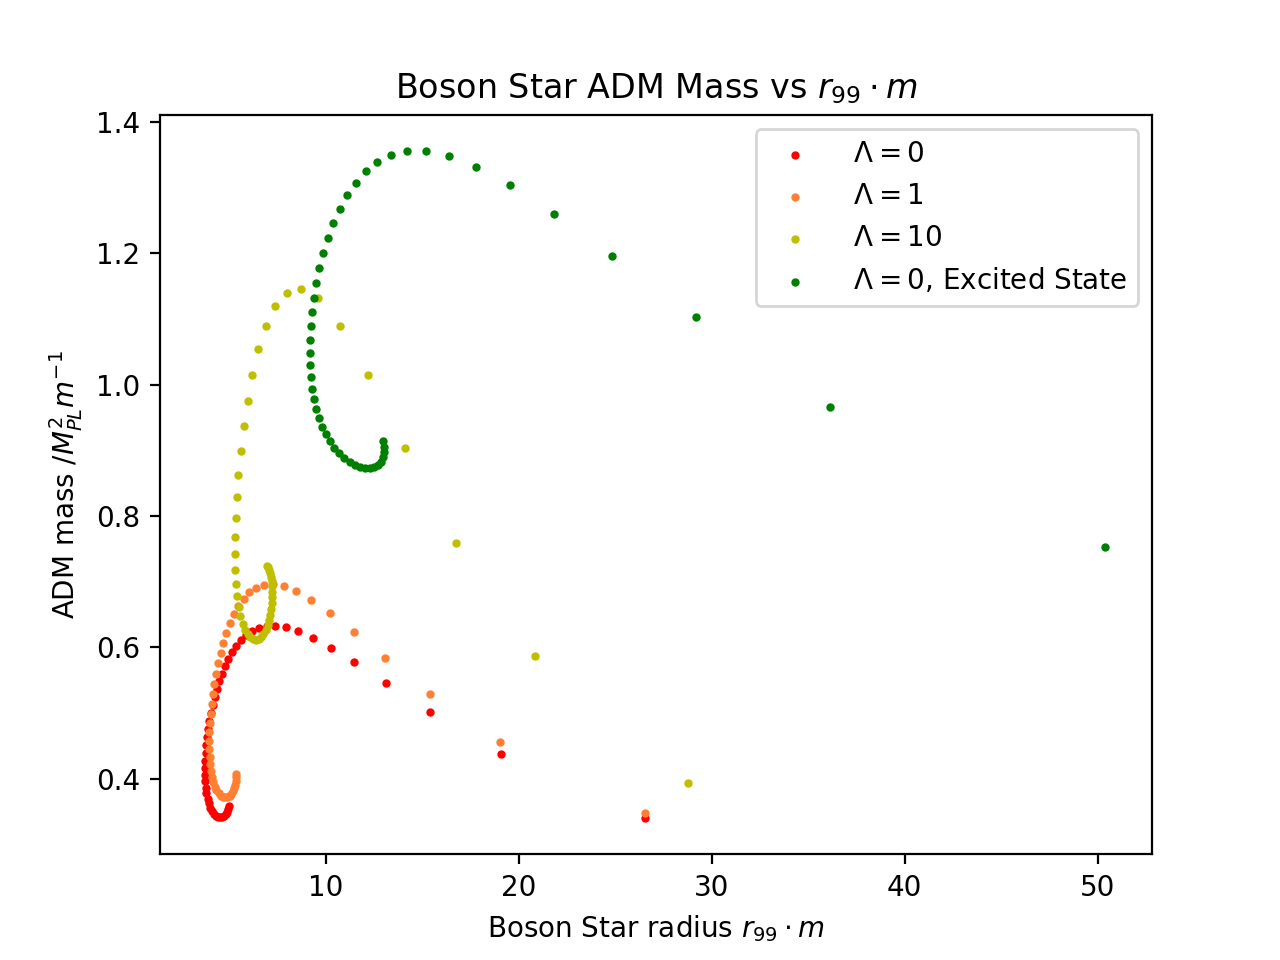
\includegraphics[width=0.8\textwidth]{png/ADM_vs_r99.png}\label{boson:fig:f2}
\end{figure}

While many different boson stars have been made to test the initial data code, all the following evolutions use the same boson star with parameters $\Lambda=0$, $\sqrt{4\pi G}\Phi(0)=0.1 \rightarrow \Phi(0) \approx 0.0282$ and ADM mass $M=0.532(7)$. This is as the stars are heavy enough to form black holes under collisions and large deformations, but stable enough to not collapse to a black hole for moderate perturbations.


EXPLAIN EIGENVALUES AND GROUND STATES BETTER.



\subsection{Single Star Evolution}
  \begin{figure}[h!]
  \caption{Left: 2D slice of initial $|\vp|$, Right: Maximum of $|\vp|$ during evolution.}
  \centering
  \subfloat{\includegraphics[width=0.5\textwidth]{mod_phi_nice0000.png}\label{boson:fig:f5}}
  \hfill
  \subfloat{\includegraphics[width=0.5\textwidth]{modphimax.png}\label{boson:fig:f6}}
\end{figure}
The first simulation done was of the $\Phi(0)=0.02820$ mini boson star; as mentioned before all simulations are done with this star. The star is supposed to remain in the centre of the grid and not change as it is a rest frame soliton; this is observed through evolution with GRChombo. Figure () shows a rough initial phase in $|\vp|$ which changes significantly upon changing the AMR regridding, hence it is likely only a side effect of the interpolation errors at the boundary of AMR regions. Figure () shows that the star conserves $\mathcal{N}$ upto 4 figures and the constraint $\mathcal{H}$ is driven towards zero as desired.

  \begin{figure}[h!]
  \caption{Left: Total Noether charge $\mathcal{N}$ during evolution, Right: $|| \mathcal{H} ||_2$ during evolution.}
  \centering
  \subfloat{\includegraphics[width=0.5\textwidth]{N.png}\label{boson:fig:f7}}
  \hfill
  \subfloat{\includegraphics[width=0.5\textwidth]{H.png}\label{boson:fig:f8}}
\end{figure}



\subsection{Superposition of Initial Data}
In order to simulate a spacetime consisting of two stars (or a star and a black hole) we must choose a way of superposing the initial data of two objects, centred at $x^{(1)}$ and $x^{(2)}$. For some field $\psi^{(j)}$ associated with the compact object at $x^{(j)}$,
\begin{equation}
\psi^{(j)} = \psi(x-x^{(j)}),
\end{equation} where $\psi$ refers to the object centred about the origin.
Taking two compact objects with fields $\vp$, $\Pi$, $\gamma_{ij}$, $\K_{ij}$, $\alpha$ and $\beta^i$, a naive superposition scheme was chosen;
\begin{align}
 \vp &= \vp^{(1)} + \vp^{(2)},\\
\Pi &= \Pi^{(1)} + \Pi^{(2)},\\
 \K^i_j &= {\K^{(1)}}^i_j+{\K^{(2)}}^i_j,\\
 \gamma_{\mu\nu} &= \gamma^{(1)}_{\mu\nu} + \gamma^{(2)}_{\mu\nu},\\
\beta_i &= \beta^{(1)}_i + \beta^{(2)}_i ,\\
 \alpha &= \sqrt{\alpha_{(1)}^2 + \alpha_{(2)}^2-1},\\
 \chi &= \det{\gamma^{(1)}_{\mu\nu} + \gamma^{(2)}_{\mu\nu}}^{-1/3},
 \end{align}
where the super-scripts ${}^{(1)}$ and ${}^{(2)}$ refer to the separate compact objects. The extrinsic curvature is chosen to be superposed with mixed indeces so that it implies the trace $\mathcal{K}$ is also superposed. If one of the compact objects is a black hole the lapse $\alpha \rightarrow 0$ on the horizon; this is circumvented by setting,
\begin{equation} \alpha = \sqrt{\chi},\end{equation}
ensuring that the lapse is real and non-negative for a all of $\Sigma_t$. Superposing two solutions in general relativity usually no longer satisfies the Einstein equation, the Hamiltonian constraint Eq.~(\ref{nr:eq:ham}) and momentum contraints Eq.~(\ref{nr:eq:mom}) are violated. For asymptotically flat compact objects, the constraint violation reduces to zero as the object separation tends to inifinity. In the case of finite separations, the CCZ4 scheme in section \ref{nr:sec:ccz4} aims to drive the constraint violation towards zero and hence a true solution of Einstein's equation. The preliminary test of collisions of compact objects in sections [REF] use this naive superposition scheme. Section [REF] explores a technique to improve the naive superposition of compact objects.



\subsection{Head-on Collisions}
All the cases studied here are for stationary initial data $\tilde{\A}_{ij}=0,\K=0$ in-falling from an initial separation of $d \cdot m = 32$ due to gravitational attraction. Firstly we consider the equal mass Boson star binary, initial data in figure (). At first they slowly infall creating a short lived object with three maxima, shown in figure (,left), then collapse to a black hole with a decaying spherical harmonic cloud (figures ) outside. As with all the simulations from now on we assume a black hole forms if $\chi \ll 16^{-1}$ where $\chi=16^-1$ is the value taken on the horizon for the isotropic Schwarzschild metric.
  \begin{figure}[h!]
  \caption{Initial Data, Left: $\chi$, Right: $|\vp|$.}
  \centering
  \subfloat{\includegraphics[width=0.5\textwidth]{headon_bs/chi0000.png}\label{boson:fig:f9}}
  \hfill
  \subfloat{\includegraphics[width=0.5\textwidth]{headon_bs/modphi0000.png}\label{boson:fig:f10}}
\end{figure}
  \begin{figure}[h!]
  \caption{Scalar field amplitude before and after black hole formation, Left: Time $t\cdot m = 150$, Right: Time $t \cdot m = 200$.}
  \centering
  \subfloat{\includegraphics[width=0.5\textwidth]{headon_bs/modphi0003.png}\label{boson:fig:f11}}
  \hfill
  \subfloat{\includegraphics[width=0.5\textwidth]{headon_bs/modphi0004.png}\label{boson:fig:f12}}
\end{figure}
   \begin{figure}[h!]
  \caption{Real part of scalar field after black hole formation, Left: xy plane, Right: yz plane, perpendicular to initial star separation.}
  \centering
  \subfloat{\includegraphics[width=0.5\textwidth]{headon_bs/phi_re0004.png}\label{boson:fig:f13}}
  \hfill
  \subfloat{\includegraphics[width=0.5\textwidth]{headon_bs/phi_re_perp0004.png}\label{boson:fig:f14}}
\end{figure}
 
The second case considered is the same Boson star outside a black hole parameterised by $M=10M_{BS}$ where $M_{BS}$ is the ADM mass of the Boson star. The scalar field tidally deforms into an ellipsoid with high central density, well beyond Kaup limit of $\vp(0)\sim 0.0764$, and spontaneous collapse to a smaller external black hole is observed. After collapse, figure (), there is an elongated cloud about the new small black hole; there are many nodal lines in $\mathrm{Re}(\vp)$ which focus on the large black hole showing the cloud is in-falling.

  \begin{figure}[h!]
  \caption{Initial Data, Left: $\chi$, Right: $|\vp|$.}
  \centering
  \subfloat{\includegraphics[width=0.5\textwidth]{LMR/chi0000.png}\label{boson:fig:f15}}
  \hfill
  \subfloat{\includegraphics[width=0.5\textwidth]{LMR/modphi0000.png}\label{boson:fig:f16}}
\end{figure}
  \begin{figure}[h!]
  \caption{Final Data at time $t\cdot m = 125$, Left: Conformal factor $\chi$, Right: Scalar field modulus $|\vp|$, Bottom: Real part of scalarfield $\mathrm{Re}(\vp).$}
  \centering
  \subfloat{\includegraphics[width=0.5\textwidth]{LMR/chi0005.png}\label{boson:fig:f17}}
  \hfill
  \subfloat{\includegraphics[width=0.5\textwidth]{LMR/modphi0005.png}\label{boson:fig:f18}}
  \\
   \subfloat{\includegraphics[width=0.5\textwidth]{LMR/phi_re0000.png}\label{boson:fig:f19}}
\end{figure}
Final case consists of an equal mass Black Hole and Boson Star, initial configuration in Figure 11. As can be seen from the plot of $\Re(\phi)$ and $|\phi|$, in Figure 12, most of the star falls into the black hole, however some scalar field manages to excite an intricate spherical harmonic cloud pattern.
  \begin{figure}[h!]
  \caption{Initial data for equal mass Boson Star and Black Hole, Left: $\chi$, Right: $|\vp|$}
  \centering
  \subfloat{\includegraphics[width=0.5\textwidth]{headon/chi0000.png}\label{boson:fig:f20}}
  \hfill
  \subfloat{\includegraphics[width=0.5\textwidth]{headon/mod_phi0000.png}\label{boson:fig:f21}}
\end{figure}
  \begin{figure}[h!]
  \caption{Time $t\cdot m=905$ for equal mass Boson Star and Black Hole, Left: $\Re(\vp)$, Right: $|\vp|$}
  \centering
  \subfloat{\includegraphics[width=0.5\textwidth]{headon/phi_re0000.png}\label{boson:fig:f22}}
  \hfill
  \subfloat{\includegraphics[width=0.5\textwidth]{headon/mod_phi0007.png}\label{boson:fig:f23}}
\end{figure}

In all three cases, the Noether charge drops rapidly upon the formation of a black hole; this will be explained in the next section. However some scalar field lingers after collapse, in each case the hair takes the form of spherical harmonics discussed in (). Also observed is the decay of the spherical harmonics to zero amplitude in these simulations with no angular momentum. 
 
\subsection{Binary Inspiral}
The only considered case here is the Quasi-circular orbit and inspiral of two equal mass boson stars. The initial boosts were determined by a newtonian calculation yielding 
\begin{equation} v^2 = \frac{M}{2d}\end{equation}
where $M=0.53(29)$ is the ADM mass of the Boson Star and d is the initial separation. For a relatively low separation of $d\cdot m =32$ code units, shown in Figures 13,14 (Left), we get $v \sim 0.0915$. The boson stars are observed to complete roughly half an orbit before merging and collapse, forming a black hole. Here a Kerr black hole is assumed to have formed as the spacetime has a significant angular momentum which should partially infall with the scalar field. 

  \begin{figure}[h!]
  \caption{Boson Star $|\vp|$. Left: initial data, Right: later time $t \cdot m = 700$}
  \centering
  \subfloat{\includegraphics[width=0.5\textwidth]{inspiral/mod_phi_inspiral_nice0000.png}\label{boson:fig:f24}}
  \hfill
  \subfloat{\includegraphics[width=0.5\textwidth]{inspiral/mod_phi_inspiral_nice0002.png}\label{boson:fig:f25}}
\end{figure}
  \begin{figure}[h!]
  \caption{Boson Star $\Re(\vp)$. Left: initial data, Right: later time $t \cdot m = 700$}
  \centering
  \subfloat{\includegraphics[width=0.5\textwidth]{inspiral/phi_inspiral_nice0000.png}\label{boson:fig:f26}}
  \hfill
  \subfloat{\includegraphics[width=0.5\textwidth]{inspiral/phi_inspiral_nice0002.png}\label{boson:fig:f27}}
\end{figure}
  \begin{figure}[h!]
  \caption{Left: Total Noether charge $\mathcal{N}$ during evolution, Right: $\Psi_4$ over 22 harmonic during evolution.}
  \centering
  \subfloat{\includegraphics[width=0.5\textwidth]{inspiral/N.png}\label{boson:fig:f28}}
  \hfill
  \subfloat{\includegraphics[width=0.5\textwidth]{inspiral/GW.png}\label{boson:fig:f29}}
\end{figure}
Figure 15 shows the total Noether charge, which is no longer conserved. When the black hole forms, the in-falling scalar field moves towards zero radius and gets hugely compressed. The huge compression causes extreme field gradients which induces continuous regridding in the AMR, but this is capped at 7 layers in this simulation to make runtime feasible. When the 8th AMR level is needed it is simply not added and resolution becomes low enough that any Noether charge near the centre is so under-resolved that it seems to fall between the gridpoints. Interestingly, Figures 13,14 (Right) show a scalar field configuration lingering around the black hole, mostly outside the contour $\chi=0.7$, looking like scalar hair. Also Figure 15 (Left) of the Noether charge appears to take significantly longer to decay than in the linear collision simulations. It can be seen in Figure 14 in the plot of $\Re(\vp)$ that the cloud has angular nodes corresponding to angular momentum similarly to boosted stars picking up nodal planes perpendicular to momentum and Figure 10 (Bottom) of the infalling cloud. 

The gravitational wave (GW) signal can be seen in Figure 15 (Right), extracted at a radius $r \cdot m = 90$. At the time $t \cdot m \approx 700$ the gravitational wave signal due to the merger appears; in order to record a longer inspiral simulations with larger initial separations need to be simulated. Currently there appears to be some small problem with the initial data, also observed in the collisions with no angular momentum, that manifests itself in noisy GW extraction and the Hamiltonian constraint initially sharply rising. 

  \subsection{STUFF}
  I think I want a stationary star
  headon collision
  maybe collison with angular momentum
  collision of bs with bh